\chapter{Data and simulation samples}

\label{ch:dataAsimulation}
\vspace{-20pt}
In this measurement, I use MINERvA data collected during antineutrino-dominated medium energy (ME) physics runs with the antineutrino flux peaked near $6$ GeV, recorded between June 29th, 2016 and February 26th, 2019. The measurement utilises the minervame5A, \mbox{minervame6A--6J} `playlists', which are lists of MINERvA runs and subruns that correspond to a specific detector configuration. This amounts to the total data exposure of $1.12 \times 10^{21}$ protons on \mbox{target (POT).} 

The analysis employs Monte Carlo (MC) simulation to try to describe the underlying antineutrino interaction physics, estimate backgrounds, characterise detector inefficiencies, evaluate systematic uncertainties, and perform various other studies. It corresponds to the detector configuration of the data-taking periods described above. The simulated MC POT is equivalent to more than \mbox{$4 \times$ data POT}, i.e. $4.96 \times 10^{21}$ POT, to reduce the statistical fluctuations in the simulation. In order to compare the simulation to data, the simulation distributions are scaled by the ratio of the data POT to the simulated MC POT, so-called POT-normalised. 

The MC encapsulates the simulation of the NuMI antineutrino beam, the antineutrino interactions in the nucleus, the environment of the nucleus itself and how it affects particles exiting it, and the propagation of the final-state particles through the MINERvA detector. For further discussion in Chapter~\ref{ch:analysis1D}, it is important to emphasise that antineutrino interactions are only simulated in the nuclear targets and tracker of the MINERvA detector, excluding the electromagnetic and hadronic calorimeter.

\section{Flux simulation} \label{sec:fluxSimulation}
% say that flux simulation is described in the NuMI chapter
% in-situ measurements
% nuclear target correction
% Combined constraint: https://arxiv.org/pdf/2209.05540.pdf
% Neutrino mode: https://journals.aps.org/prd/pdf/10.1103/PhysRevD.100.092001
% IMD: https://arxiv.org/abs/2107.01059

\begin{figure}[b!]
  \centering
  {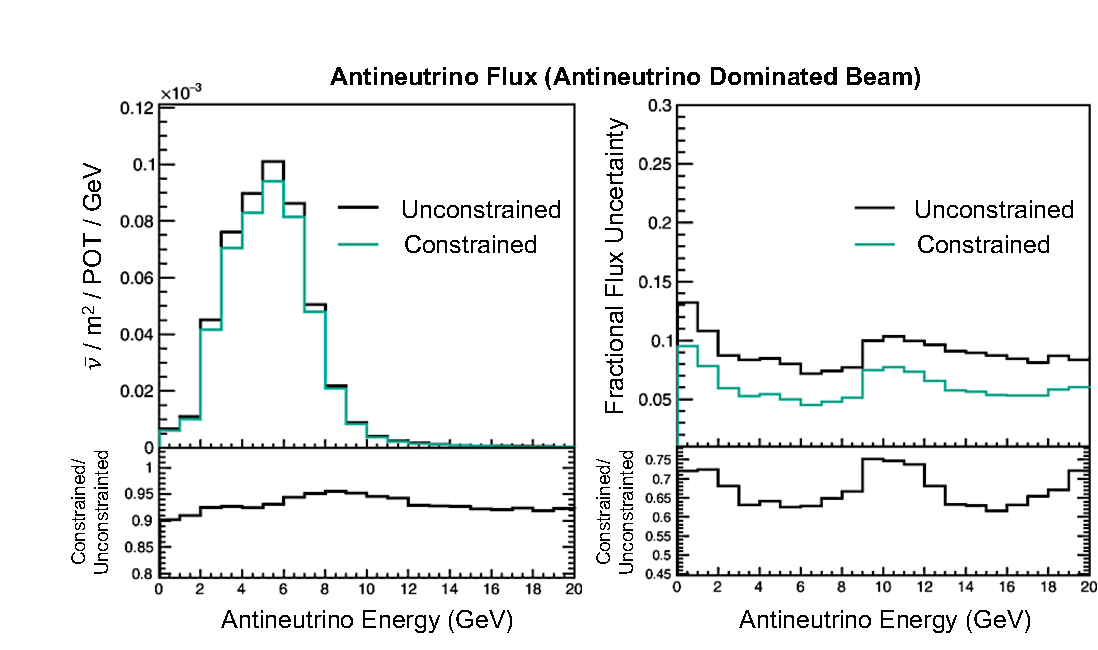
\includegraphics[width=1\textwidth]{05dataAsimulation/figures/fluxConstraint.pdf}}%
  \caption{Left: Predicted antineutrino flux in bins of antineutrino energy before and after constraining the \textit{a priori} model using the (anti)-neutrino electron scattering and inverse muon decay \textit{in-situ} measurements. Right: Fractional flux uncertainty on the predicted antineutrino flux before and after the constraint. Plots adapted from Ref.~\cite{Zazueta2023_PhysRevD.107.012001}. }
  %[short caption] {long caption}
  \label{fig:fluxConstraint}
\end{figure}
  

The simulation begins with the base antineutrino flux simulation constrained by external hadron production data described in Section~\ref{sec:NuMI}. The flux model in this analysis is further improved by \textit{in-situ} measurements of processes with known cross-sections, specifically the (anti)neutrino-electron elastic scattering \cite{Valencia2019_PhysRevD.100.092001,Zazueta2023_PhysRevD.107.012001} and inverse muon decay \cite{Ruterbories2021_PhysRevD.104.092010}.

% can be both muon neutrino (CC t-channel) and electron neutrino (NC and CC s-channel)
The (anti)neutrino-electron elastic scattering, $\nu e^{-}\rightarrow\nu e^{-}$, is a well understood, purely leptonic process. Therefore, its cross-section can be predicted to a very high precision using the Standard Model electroweak theory. The (anti)neutrino-electron elastic scattering events are relatively rare with cross-section three orders of magnitude smaller than (anti)neutrino-nucleus scattering. However, due to their distinct experimental signature of very forward electromagnetic showers with no other activity, they can be selected with only a few background events.\enlargethispage{2\baselineskip}~The discrepancies between the data and MC in the electron energy spectrum can be interpreted as mismodelling of the flux distribution, providing a constraint on the normalisation of the flux and thus the peak of the flux.~MINERvA measured the (anti)neutrino-electron elastic scattering electron energy spectra in both ME neutrino and antineutrino dominated beams physics runs \cite{Valencia2019_PhysRevD.100.092001,Zazueta2023_PhysRevD.107.012001}. 

The inverse muon decay (IMD), $\nu_{\mu}e^{-}\rightarrow\mu^{-}\nu_{e}$, is another leptonic process which was measured by MINERvA in order to constrain the flux \cite{Ruterbories2021_PhysRevD.104.092010}. It can be identified by a very forward-going high-energy muon. IMD has (anti)neutrino energy threshold of \mbox{$\approx 11$ GeV}. Hence, it provides insight into the high-energy tail of the flux, in which phase space is mostly dominated by (anti)neutrinos produced by underfocused or unfocused $K^+$ \mbox{and $\pi^{+}$}. 

This analysis uses MINERvA's combined flux constraint of (anti)neutrino-electron scattering and IMD \cite{Zazueta2023_PhysRevD.107.012001} whose impact is shown in Figure \ref*{fig:fluxConstraint}. The single normalisation constraint was extracted using Bayes' theorem, where the posterior probability is given by the prior flux prediction multiplied by the likelihood of the electron spectra measurement given the \textit{a priori} model. The \textit{a priori} flux uncertainty is estimated using the multiverse method \cite{MAT_Messerly_2021}, where an ensemble of flux predictions, so-called universes, is created by varying flux parameters within their uncertainties. The procedure takes into account the correlations between the predictions of the number of events. 

The flux simulation is then reweighted by the ratio of the weighted average of post-constraint flux universes to the weighted average of pre-constraint fluxes. The procedure results in predictions from universes with poor data agreement to be weighted down, which reduces the uncertainty (spread of the universes). In antineutrino dominated beam, the antineutrino energy range integrated flux uncertainty is reduced from $7.8\%$ to $4.7\%$ \cite{Zazueta2023_PhysRevD.107.012001} as shown in Figure \ref*{fig:fluxConstraint} and is further discussed in Chapter~\ref{ch:systematics}.

\subsection{Nuclear target flux} \label{sec:nuclear_target_flux}

% Figures:
% calculated flux in targets + ratio (antineutrinos)
% point to neutrinos in a reference
% Flux in individual petals figure
% Figure of the individual petals in a hexagon
% Regularisation curve for targets in the back-up
% back-up: antineutrino energy flux in 2D rebinning
% weights before and after in the back-up for carbon, maybe get others 
% table of chi2 in the back-up

While the antineutrino beam is focused as described in Section~\ref{sec:NuMI}, the transverse distribution of the beam is relatively wide. Additionally, due to the downward pointing of the NuMI beam with respect to MINERvA, this also affects the flux seen by the detector as a function of the longitudinal position.\enlargethispage{1\baselineskip} The flux distribution described above provides an accurate representation of the averaged flux in the active tracker region and correctly accounts for these effects. However, the complex geometry of the nuclear target region, as detailed in Section~\ref{sec:MINERvAdetector}, with varying transverse positions of different materials within individual targets, particularly off-centre of the detector and, consequently, off-centre of the beam, is expected to introduce variations in both shape and normalisation of the flux compared to the tracker.

The nuclear target flux differences in the neutrino beam were first taken into consideration in cross-section calculations in Refs.~\cite{KleykampThesis2021, KleykampCCQE_PhysRevLett.130.161801} with applied neutrino-electron elastic scattering flux constraint only. To enable flux-independent comparisons between nuclear targets, i.e.~the nuclear target-to-scintillator cross-section ratios as discussed in Chapter~\ref{ch:measurement}, the procedure in Refs.~\cite{KleykampThesis2021, KleykampCCQE_PhysRevLett.130.161801} extracts the scintillator tracker cross-section in different transverse regions of the MINERvA fiducial volume. It is then weighted so that the summed scintillator cross-section has the same effective flux as the target flux.

\begin{figure}[b!]
  \centering
  \vspace{5pt}
  {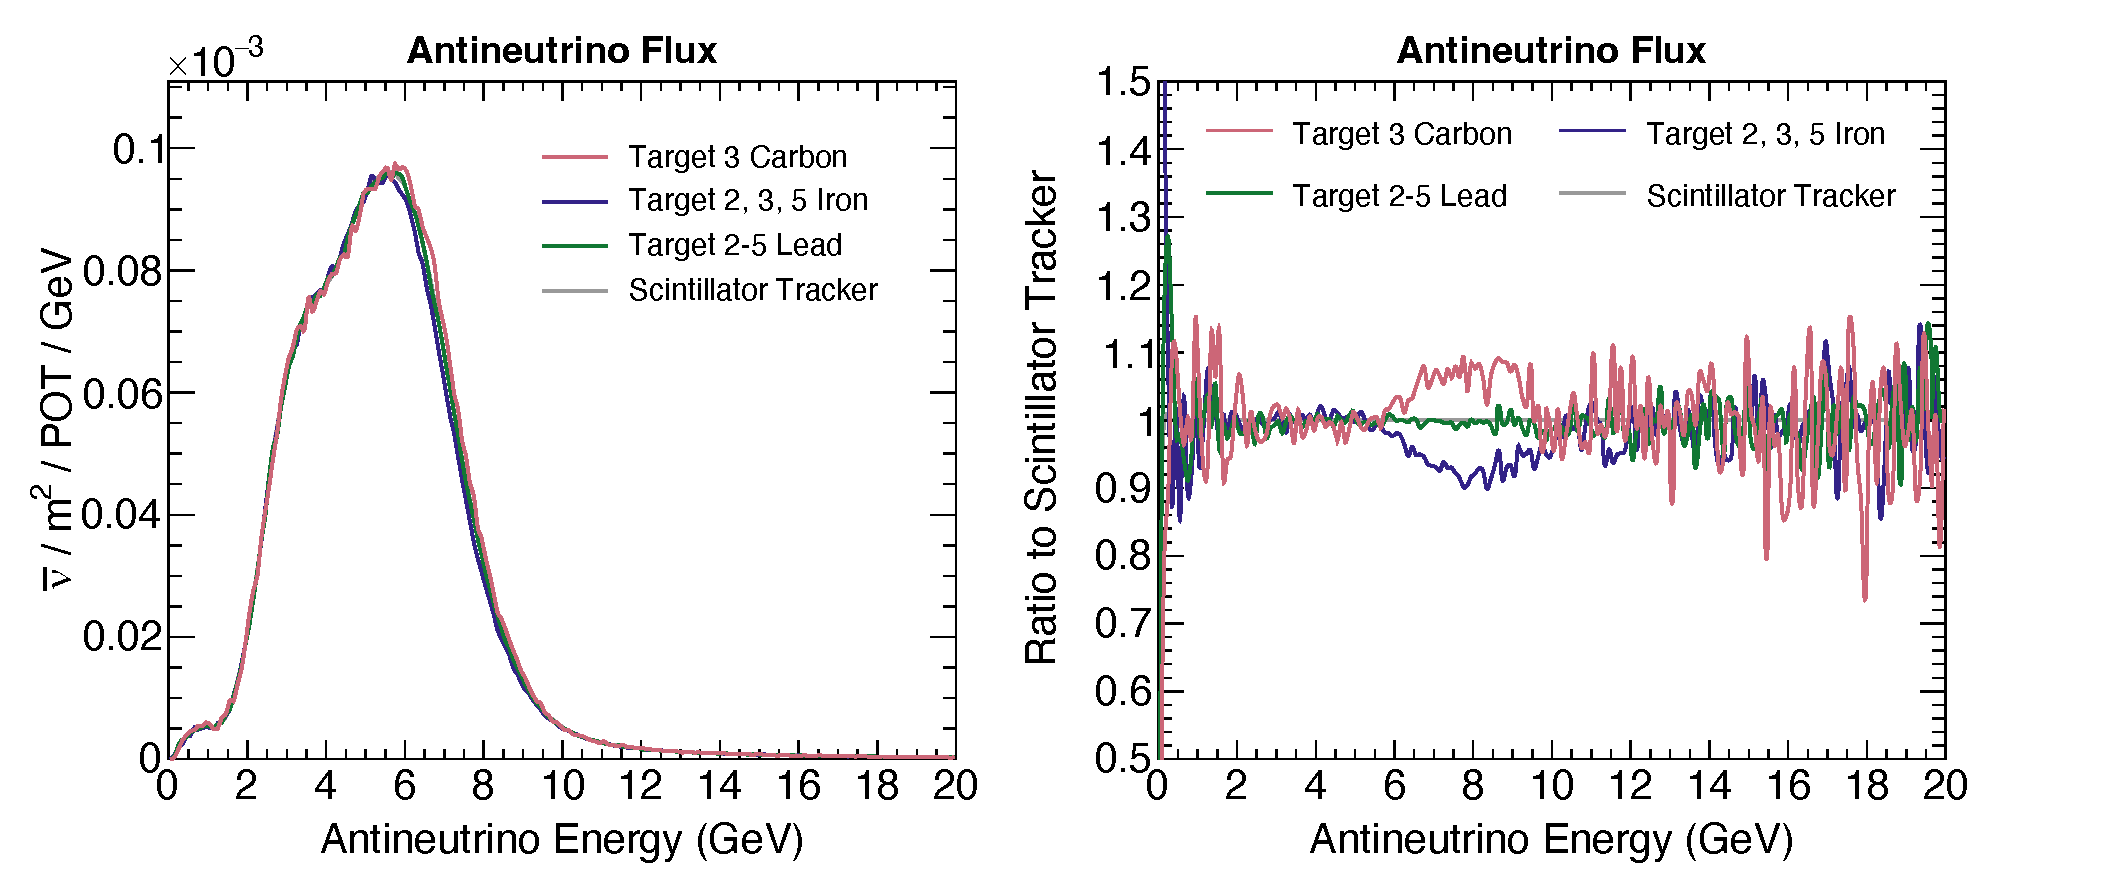
\includegraphics[width=1.01\textwidth]{05dataAsimulation/figures/nuclearFlux.pdf}}%
  \caption{Left: Calculated antineutrino flux for carbon, iron, and lead compared to the scintillator tracker flux. Right: Nuclear target-to-scintillator tracker flux ratio illustrating the flux differences in the 6--10~GeV region.}
  %[short caption] {long caption}
  \label{fig:nuclearFlux}
\end{figure}

I extended the procedure to the antineutrino flux with MINERvA's combined flux constraint of (anti)neutrino-electron scattering and IMD, and simultaneously reimplemented the neutrino flux with this new flux constraint as well. The antineutrino fluxes for each nuclear target (or combined nuclear targets of the same material) were calculated, as detailed in Appendix~\ref{ch:appendix_NuclearTargetFlux}, using the true information from the simulation.\enlargethispage{1\baselineskip}

Figure~\ref{fig:nuclearFlux} depicts the calculated antineutrino fluxes for the combined nuclear targets used in this work and their ratios to the scintillator tracker flux distribution. Generally, the nuclear target fluxes differ by up to 10\% in the 6--10~GeV region (the falling edge of the flux peak). If the average position of the target is above the centre of the beam, as is the case for carbon, the nuclear target flux is higher than that for the scintillator. Conversely, if the average position of the target is below the centre of the beam, as is the case for the combination of iron targets, the nuclear target flux is lower than that for the scintillator. The combination of lead targets has approximately the same centre of mass and shape as the tracker, thus resulting in a flat lead-to-scintillator flux ratio.

\begin{figure}[b!]
  \centering
  \vspace{-10pt}
  {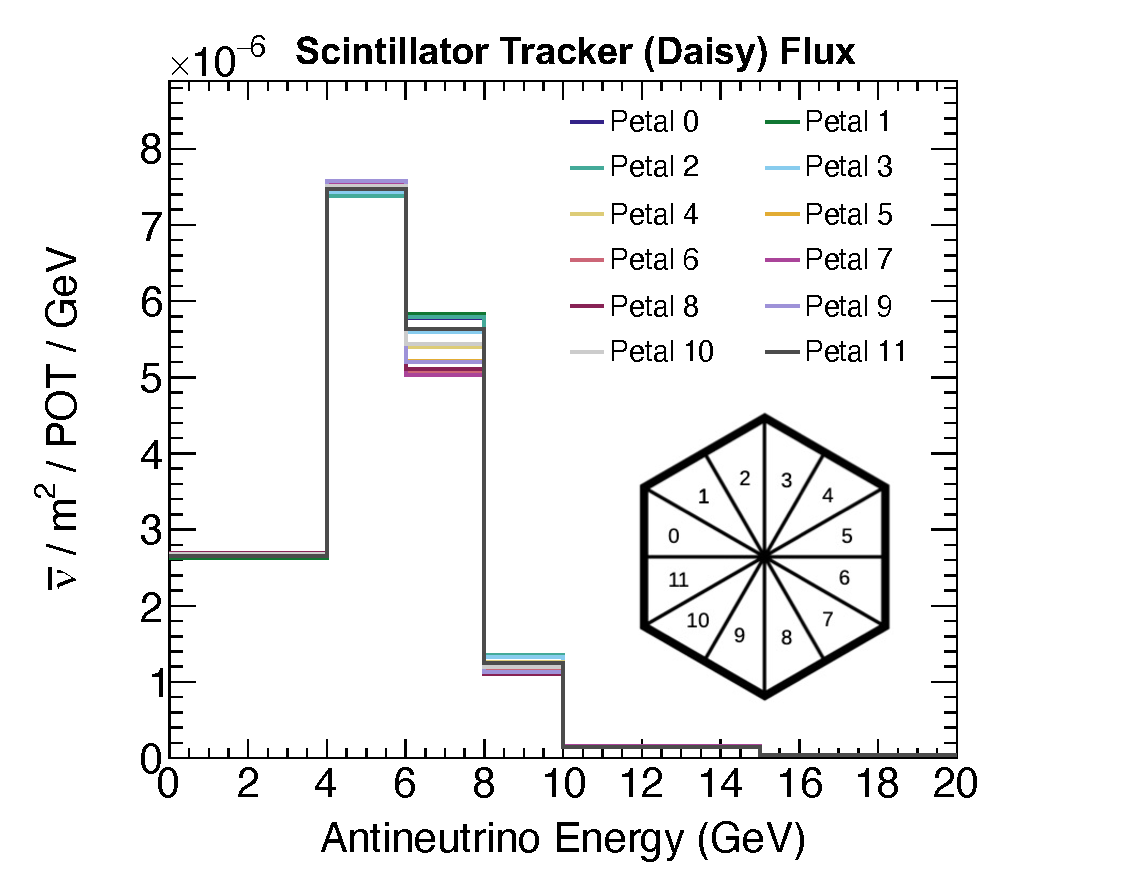
\includegraphics[width=0.8\textwidth]{05dataAsimulation/figures/daisyPetals.pdf}}%
  \caption{Antineutrino scintillator tracker flux for each ‘daisy petal' as a function of antineutrino energy. The hexagon insert illustrates petal positions when looking downstream of the detector.}
  %[short caption] {long caption}
  \label{fig:daisyPetals}
\end{figure}

Similarly to the nuclear target fluxes, the scintillator tracker flux can be extracted in~12~transverse bins referred to as ‘daisy petals', as illustrated in Figure~\ref{fig:daisyPetals}.~A~linear combination of these ‘daisy petal' fluxes is then taken to create an effective scintillator tracker flux that matches that of the nuclear target combination.\enlargethispage{1.5\baselineskip}~The weights for the individual petals are calculated using a regularised $\chi^{2}$ fit and later applied to the efficiency-corrected ‘daisy petal' distributions in the analysis procedure detailed in Chapter~\ref{ch:analysis1D}. Specifics of this so-called ‘daisy' reweight technique are also further described in Appendix~\ref{ch:appendix_NuclearTargetFlux}.


\section{Antineutrino simulation}
% MINERvA tune v4.3.0
% GENIE 2.12.5 with Valencia RPA applied to QE (RFG), non-resonant pion
% production reductuon to 43%, low recoil fit (LE) applied to Valencia 2p2h (50% enhancement integrated over phase space)
% Full pion bubble chamber fit (CCNormREs increased to 1.15 and MaRES set to 0.94 + correlations)
% CC1pi+ lowQ2 pion production syppression (ME) + normalization of COH using the angle and energy of the pion with highest kinetic energy
% - applied to resonant and DIS events with W < 1.4 GeV with single pion multiplicity - antineutrino case applied to pi- instead of pi+
% Resonant and DIS the larget contribution to the inclusive ME sample

% Nuclear model
% Interacion model
% Quasi-elastic scattering
 % Valencia RPA
% Multi-nucleon scattering
    % Valencia 2p2h 
    % LE Fit
% Pion production
  % Resonant pion production 
    % Full pion bubble chamber fit
  % Non-resonant pion production
    % Non-resonant pion production reduction
  % Coherent pion production
    % normalization
% Deep inelastic scattering
% Final state interactions

MINERvA uses the (anti)neutrino interaction event generator GENIE (Generates Events for Neutrino Interaction Experiments) version 2.12.6 \cite{genie_ANDREOPOULOS201087,genie_andreopoulos2015}. It models how often (anti)neu\-tri\-nos from NuMI interact with nuclei in MINERvA and what are the underlying interaction physics processes. It also models the nuclear environment of the nucleus and how it affects the initial (anti)neutrino interaction as well as the final-state kinematics, i.e. what particles are produced in the final state. Furthermore, this analysis uses a variety of modifications to the baseline antineutrino simulation to better describe MINERvA data. These are applied as weights to each event, effectively scaling the probability of the event occurring based on the fit to the experimental data.
% GENIE https://arxiv.org/abs/0905.2517
% GENIE https://arxiv.org/abs/1510.05494

\subsection{Nuclear model}

As the incoming antineutrino in most cases interacts with the constituents of the nucleus~(nucleons or quarks), the simulations need to account for the effects of the nuclear environment. GENIE models the nucleus as a relativistic Fermi gas (RFG) \cite{RFG_SMITH1972605}, where nucleons are confined to a potential well with walls at the nuclear radius. RFG treats the nucleons within a nucleus as independent particles (so-called impulse approximation). The nucleons inside the nucleus have a nucleus-specific flat momentum distribution between~0~and the Fermi momentum $p_{\text{F}}$ in the ground state, determined from inclu\-sive electron scattering, and binding energy $E_{\text{B}}$. The $E_{\text{B}}$ refers to the energy needed to sepa\-rate a bound nucleon from the nucleus. 

% before corrections
%needed to bring a bound nucleon on-shell and separate it from the remnant nucleus, or for the nucleus to be excited to a~higher-energy bound state. 

% RFG https://www.sciencedirect.com/science/article/pii/0550321372900405

Because nucleons are fermions, they must obey the Pauli exclusion principle resulting in Pauli blocking. In quasi-elastic interactions, the final-state nucleon has to have momentum above $p_{\text{F}}$, which significantly suppresses the cross-section at low $Q^{2}$. To account for short-range correlations between the nucleons, i.e.~interactions between the nucleons inside the nucleus, which can lead to a momentum greater than $p_{\text{F}}$, the simulation contains Bodek-Ritchie high-momentum tail \cite{BodekRitchie1981_PhysRevD.24.1400}.
% Bodek Ritchie tail https://link.aps.org/doi/10.1103/PhysRevD.24.1400

Other nuclear models are relevant in the context of certain antineutrino interaction processes and are discussed below.
%M.Martini et al. A Unified approach for nucleon knock-out, coherent and incoherent pion production in neutrino interactions with nuclei. Phys. Rev. C 80:065501 (2009).
%GENIE models the nucleus as a relativistic Fermi gas (RGF) Martini et al.

%Adapted from Carlos A. Bertulani, Nuclear physics in a nutshell,
%Princeton University Press, 2007, p. 473


\subsection{Interaction model}
As described in Chapter~\ref{ch:theory}, different types of antineutrino interactions occur at different antineutrino energies. Due to the inclusive nature of this analysis, all antineutrino interaction modes contribute to the final cross-section. However, the higher-energy inelastic components such as resonant pion production and deep inelastic scattering will be dominant in the ME sample. The antineutrino interaction model described below will be referred to as MINERvA tune v4.3.0.


\subsubsection{Quasi-elastic scattering}
Quasi-elastic interactions are simulated using the Llewellyn-Smith formalism \cite{LLEWELLYNSMITH1972261}, which factorises the cross-section as a function of the four-momentum transfer squared, $Q^2$. The quasi-elastic vector form factors are modelled using the BBBA05 parametrization~\cite{BRADFORD2006127} of the electromagnetic form factors from electron scattering experiments. The axial form factor uses the dipole form with an axial mass of $M_{A}^{\text{QE}} = 0.99$ GeV/$c^2$. In addition, MINERvA's low energy low recoil neutrino analysis shown in Figure \ref{fig:LElowRecoil_2p2hRPA} demonstrated suppression of data in the low $Q^2$ region possibly due to long-range correlations in the nucleus \cite{Rodrigues2016_PhysRevLett.116.071802}. To address this, MINERvA modifies the baseline simulation as a function of energy and three-momentum transfer based on the random phase approximation (RPA) part of the Valencia model~\cite{RPANieves2004_PhysRevC.70.055503, gran2017model}.

\begin{figure}[b!]
  \centering
  {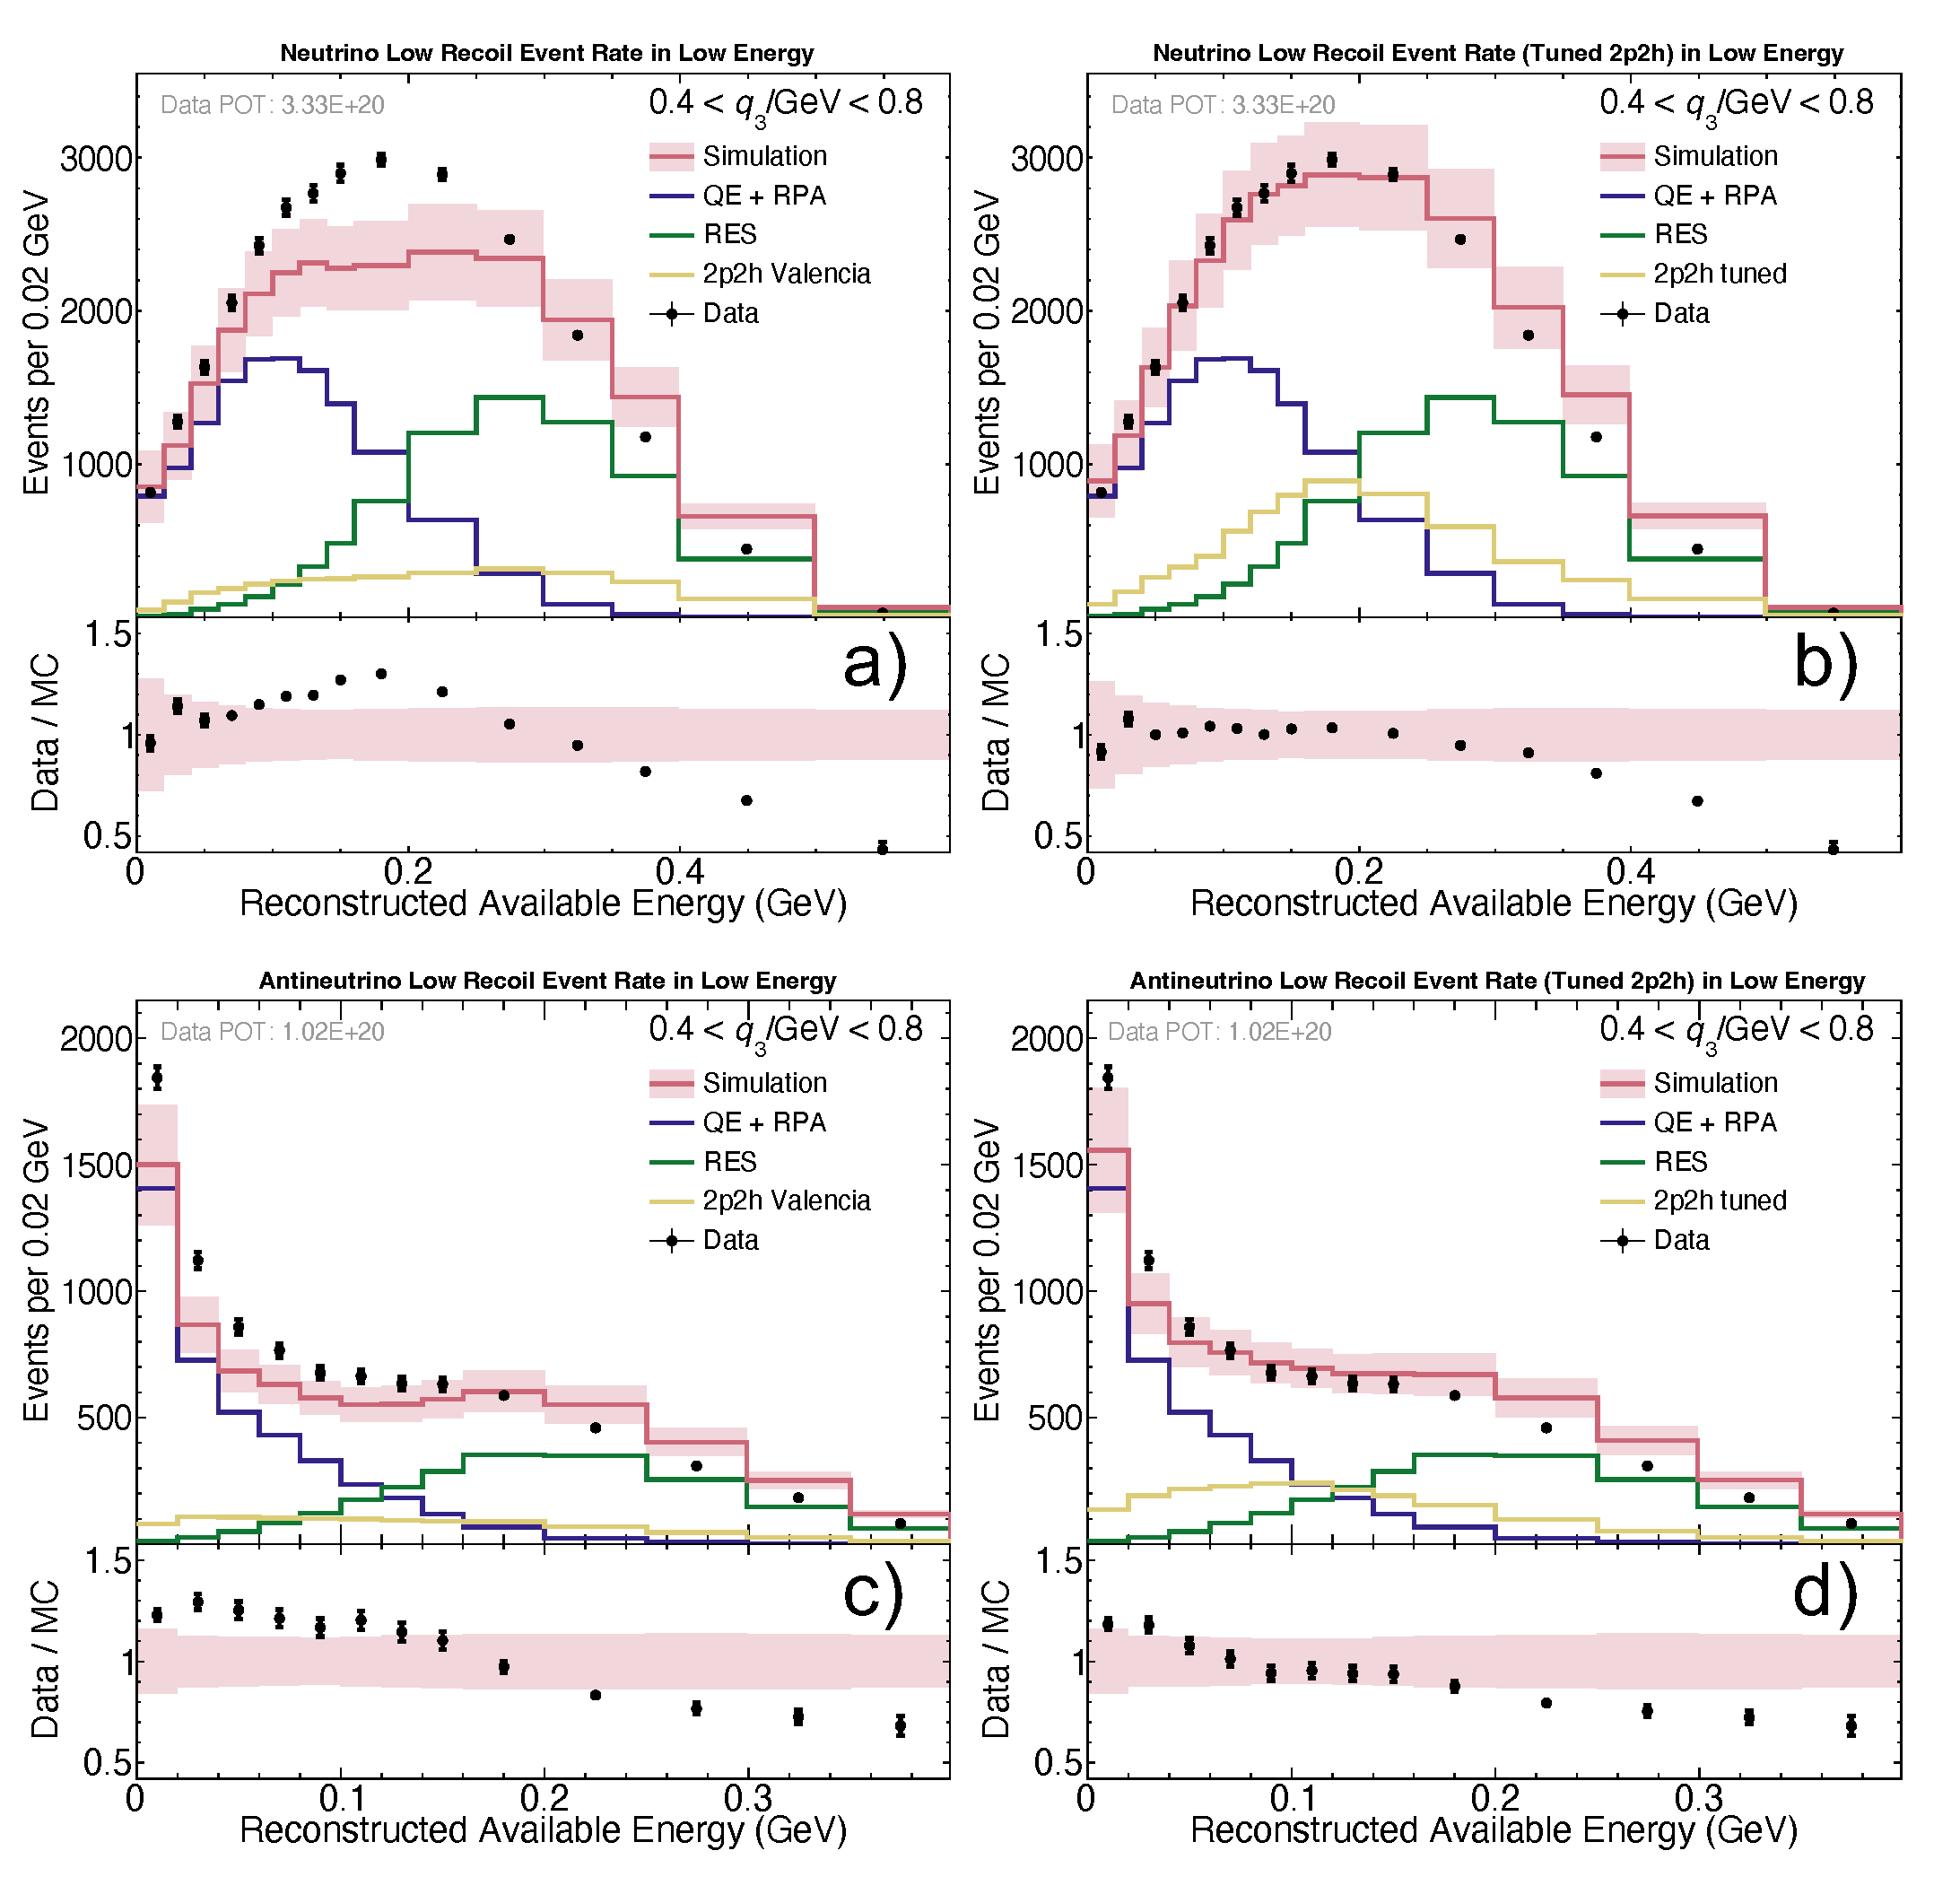
\includegraphics[width=1.01\textwidth]{05dataAsimulation/figures/LElowRecoil_2p2hRPA.pdf}}%
  \caption{MINERvA measurements of neutrino \cite{Rodrigues2016_PhysRevLett.116.071802} and antineutrino \cite{Gran2018_PhysRevLett.120.221805} low-recoil scattering in low energy as a function of reconstructed available energy, motivating the addition of RPA and 2p2h modification.~Note that the available energy corresponds to the visible recoil energy in the detector. a)~Low energy low recoil neutrino comparison of simulated and measured event rate with visible data and simulation discrepancy. b)~Improved simulation with enhanced 2p2h events shows better agreement with data. c)~Equivalent analysis in antineutrino mode compared to the base simulation. d)~Improved simulation in the antineutrino mode using the fit of the 2p2h enhancement from the neutrino mode, i.e. b), also shows better agreement with data. Furthermore, the distributions demonstrate the need for the random phase approximation (RPA) suppression in the quasi-elastic process (QE).}
  %[short caption] {long caption}
  \label{fig:LElowRecoil_2p2hRPA}
\end{figure}

% LLewellyn-Smith: https://www.sciencedirect.com/science/article/abs/pii/0370157372900105
% BBBA05: https://www.sciencedirect.com/science/article/pii/S0920563206005184
% Rodrigues: https://journals.aps.org/prl/abstract/10.1103/PhysRevLett.116.071802
% RPA Valencia model: https://arxiv.org/abs/nucl-th/0408005
% RPA Valencia model procedure: https://arxiv.org/abs/1705.02932


\subsubsection{Multi-nucleon scattering}
\label{subsec:2p2h}
Multi-nucleon scattering, specifically the 2p2h interaction, is simulated using the Valencia 2p2h model~\cite{2p2hNieves2011_PhysRevC.83.045501,2p2hGran2013_PhysRevD.88.113007,2p2hschwehr2017genie}. However, based on MINERvA's low energy recoil neutrino analysis~\cite{Rodrigues2016_PhysRevLett.116.071802}, the cross-section is increased in specific regions of energy and three-momentum transfer as shown in Figure \ref*{fig:LElowRecoil_2p2hRPA}.\enlargethispage{1\baselineskip} This results in 2p2h rate enhancement by 50\% over the nominal prediction when integrated over all phase space. Figure \ref*{fig:LElowRecoil_2p2hRPA} also shows the equivalent analysis in the antineutrino mode \cite{Gran2018_PhysRevLett.120.221805} and how the 2p2h tune (fit to neutrino data only) naturally improves the simulation prediction for the data. \vspace{20pt}



% Valencia 2p2h model: https://arxiv.org/abs/1102.2777
% Valencia 2p2h model: https://arxiv.org/abs/1307.8105
% Valencia 2p2h model in GENIE: https://arxiv.org/abs/1601.02038

% Low recoil analysis: https://journals.aps.org/prl/abstract/10.1103/PhysRevLett.116.071802
% 2p2h enahncement: https://journals.aps.org/prl/abstract/10.1103/PhysRevLett.120.221805

\subsubsection{Pion production}
\label{subsec:pionProduction}
% OG Rein-Seghal: https://www.pas.rochester.edu/~ksmcf/rein-sehgal/rein-sehgal.pdf
% GENIE documentation: https://arxiv.org/pdf/1510.05494.pdf
% How specifically imlemented and what resonances are omitted from R-S; https://journals.aps.org/prd/pdf/10.1103/PhysRevD.100.072005
% Note the resonances omitted are delta 1600 and N 1990 (quoted as 1970 in the original paper): https://pdg.lbl.gov/2011/listings/rpp2011-list-N-1990-F17.pdf
% P. Stowell's thesis is pretty good too: https://etheses.whiterose.ac.uk/22623/1/thesis.pdf

GENIE simulates the charged and neutral single pion production via baryon resonances using the Rein-Seghal (RS) model \cite{REIN198179} up to the hadronic invariant mass cut of $W$~=~1.7~GeV/$c^2$ \cite{genie_ANDREOPOULOS201087, genie_andreopoulos2015}. Out of the 18 resonances in the RS model, only 16 are included in GENIE due to $\Delta$(1600) and $N$(1990) having ambiguous experimental signatures at the time of implementation \cite{genie_ANDREOPOULOS201087, genie_andreopoulos2015}. It also does not include interference terms between the resonances and the lepton masses in the cross-section calculation. However, the effect of the latter is taken into account in calculating the phase space limits. 

%\begin{table}[ht]
%  \caption{Nonlinear Model Results}
%  \centering
%  \begin{tabular}{c c c c}
%  \hline\hline
%  Case & Method\#1 & Method\#2 & Method\#3 \\ [0.5ex] % inserts table %heading
%  \hline
%  1&50&837&970 \\
%  2&47&877&230 \\
%  3&31&25 &415 \\
%  4 & 35 & 144 & 2356 \\
%  5 & 45 & 300 & 556 \\ [1ex]
%  \hline
%  \end{tabular}
%  \label{table:nonlin}
%\end{table}

% Rein-Seghal: https://www.sciencedirect.com/science/article/abs/pii/0003491681902426?via%3Dihub
% P33 and(1640) and F17(1970) from RS model are not in GENIE: https://genie-docdb.pp.rl.ac.uk/DocDB/0000/000002/003/man.pdf p 26
% This corresponds to
% Delta 3/2 around 1630
% N 7/2 around 1970
% N has isospin of 1/2
% Delta has an isospin of 3/2

\begin{figure}[b!]
  \centering
  {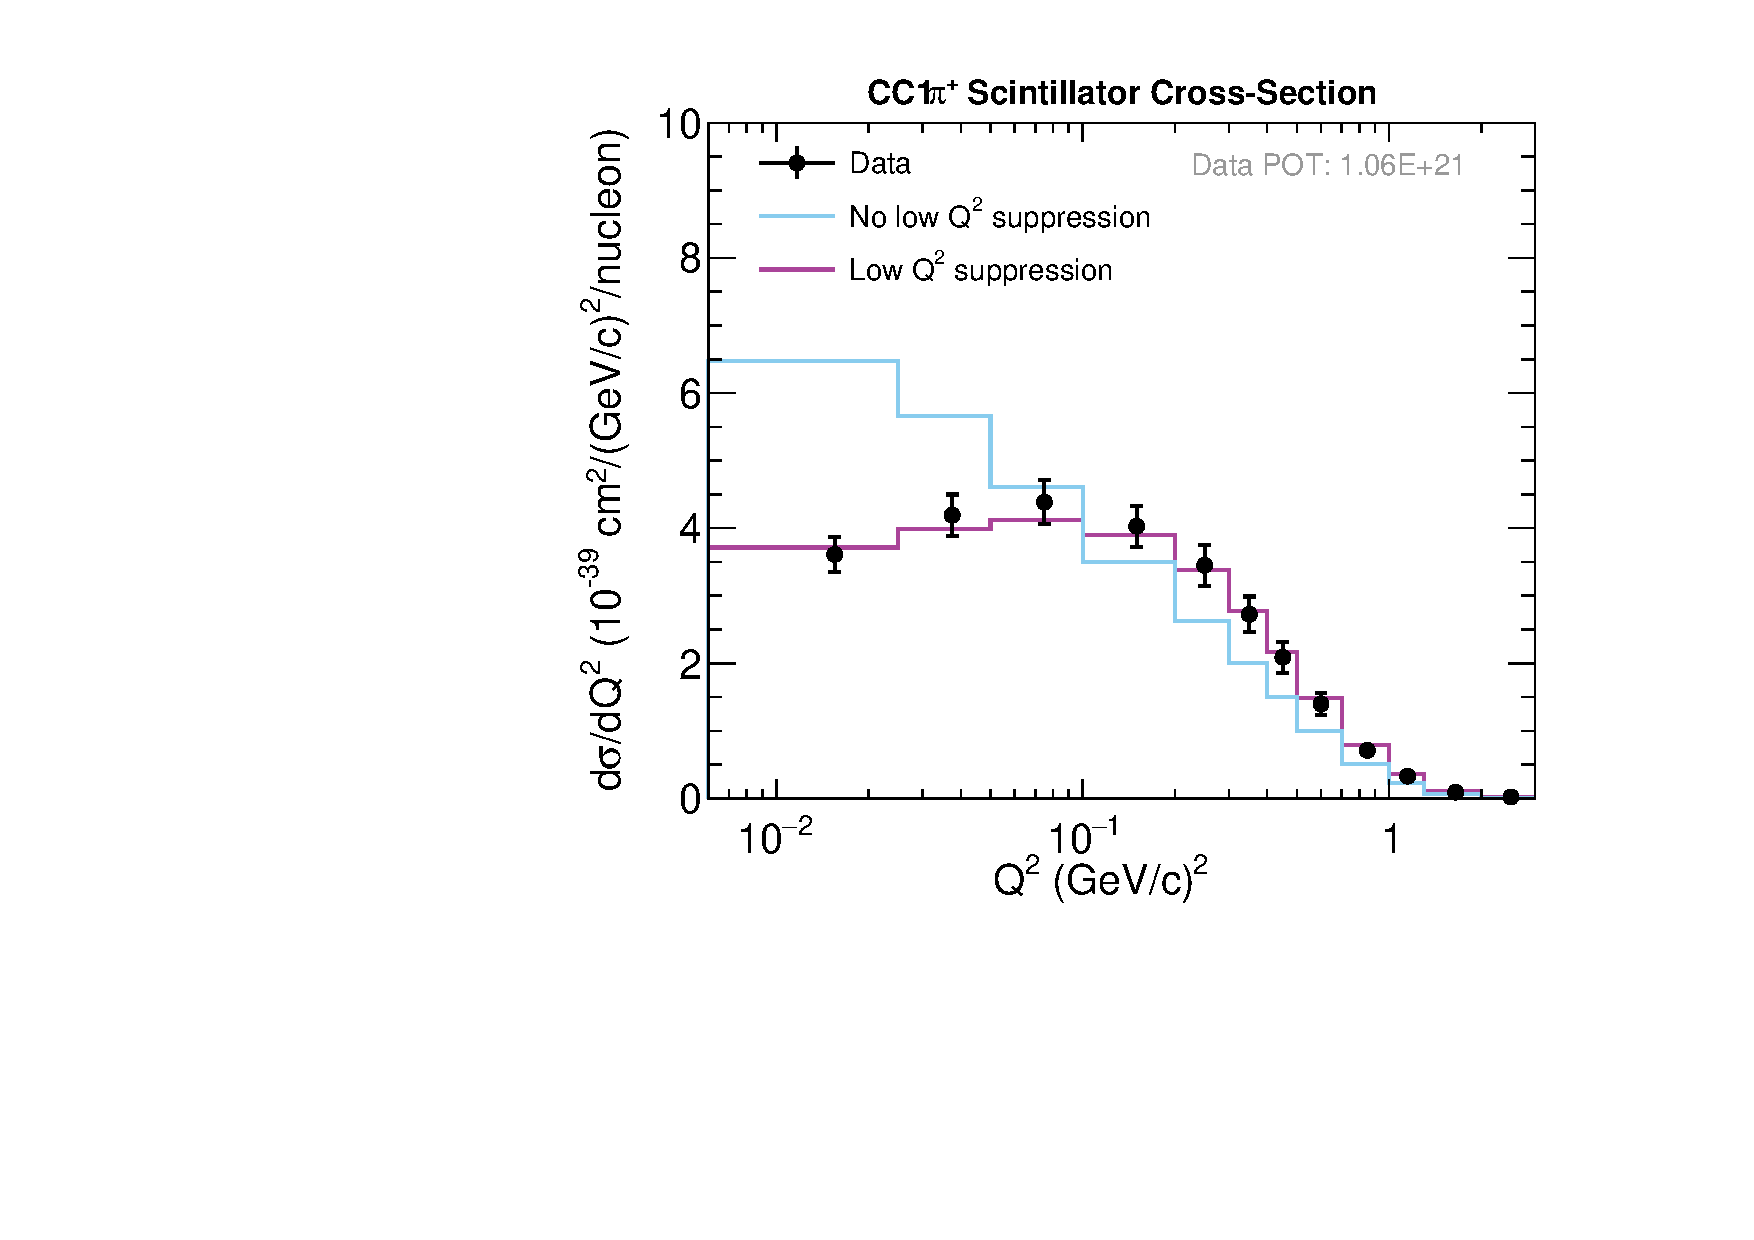
\includegraphics[width=0.8\textwidth]{05dataAsimulation/figures/lowQsup_xsec.pdf}}%
  \caption{Charged-current single pion cross-section measurement on the scintillator (data points) as a function of the four-momentum transfer squared, $Q^2$, compared to the simulation without and with the low $Q^2$ suppression. The simulated cross-section with the low $Q^2$ suppression shows better agreement with the data. Plot uses the medium energy CC1$\pi^{+} $ result \cite{Bercellie2023_PhysRevLett.131.011801}.}
  %[short caption] {long caption}
  \label{fig:lowQsup}
\end{figure}


MINERvA reweights its resonant single pion production cross-section based on a reanalysis of the deuterium bubble chamber measurements of single pion production taken by Argonne and Brookhaven National Laboratories (ANL, BNL) \cite{ANL_PhysRevD.25.1161, BNL_PhysRevD.34.2554}. The reanalysis constrained the resonant axial mass to $M_{A}^{\text{RES}} = 0.94$ GeV/$c^2$ (from its nominal value of $1.12$~GeV/$c^2$ \cite{genie_ANDREOPOULOS201087, genie_andreopoulos2015}), and set the resonant normalisation parameter to 1.15 \cite{pion_Rodrigues_2016}. 

% ANL data: https://journals.aps.org/prd/abstract/10.1103/PhysRevD.25.1161s
% BNL data: https://journals.aps.org/prd/abstract/10.1103/PhysRevD.34.2554
% reanalysis of ANL/BNL: https://arxiv.org/abs/1601.01888

% Coherent is low Q2 ~ low pT^2
The subdominant process of coherent pion production is simulated in GENIE using the coherent pion RS model \cite{coherent_REIN198329} including lepton mass terms \cite{coherentMass_REIN2007207}. It is further reweighted in both energy and the angle of a pion with the highest kinetic energy to agree with MINERvA's recent measurement of coherent pion production \cite{Ramirez2023_PhysRevLett.131.051801}. 
% Rein-Seghal coherent: https://www.sciencedirect.com/science/article/pii/0550321383900901
% RS mass correction: https://www.sciencedirect.com/science/article/pii/S0370269307012580
% MINERvA measurement: https://journals.aps.org/prl/abstract/10.1103/PhysRevLett.131.051801


% M. A. Ramirez et al. (MINERvA), ““νμ-Induced CC Coherent π+ Production from C, CH, Fe and Pb nuclei in the MINERvA Detector” (manuscript in preparation),” (2022), “νμ-Induced CC Coherent π+ Production from C, CH, Fe and Pb nuclei in the MINERvA Detector” (manuscript in preparation).
% Transition region
% Brian's thesis was useful!!! ("transition region#\")

The non-resonant pion production represents part of the transition region between the resonance (RES) and deep inelastic scattering (DIS) depicted in Figure \ref{fig:WdistribGENIE}. In GENIE, it is modelled by the scaled Bodek-Yang model \cite{BodekYang_2003, BODEK2005113} for DIS described later in this section. It is added incoherently to the resonant pion production in the region restricted by the mass of $\Delta^{++}(1232)$ resonance and \mbox{$W <$ 1.7 GeV/$c^2$} \cite{genie_ANDREOPOULOS201087,genie_andreopoulos2015}. DIS interactions with resonance-like final states such as 1$\pi$ and $2\pi$ are suppressed to avoid double counting. Additionally, MINERvA reduces the contribution of non-resonant pion production to~43\%~of its nominal value based on the ANL/BNL data reanalysis \cite{pion_Rodrigues_2016}.

% Bodek-Yang: https://arxiv.org/abs/hep-ex/0210024
  
  
Furthermore, this analysis reweights its single pion production, both resonant and non-resonant, with $\pi^-$ in final states in the \mbox{$W <$ 1.4 GeV/$c^2$} region. It applies low $Q^2$ suppression based on the medium energy charged-current 1$\pi^+$ analysis result \cite{Bercellie2023_PhysRevLett.131.011801} as shown in Figure \ref{fig:lowQsup} to events on all nuclei except hydrogen, assuming the suppression comes from interactions in the nucleus.

% Aaron's reweight: https://arxiv.org/abs/2209.07852

% Pion production
  % Resonant pion production 
    % Full pion bubble chamber fit
  % Non-resonant pion production
    % Non-resonant pion production reduction
  % Coherent pion production
    % normalization


\subsubsection{Deep inelastic scattering}

\begin{figure}[b!]
  \centering
  {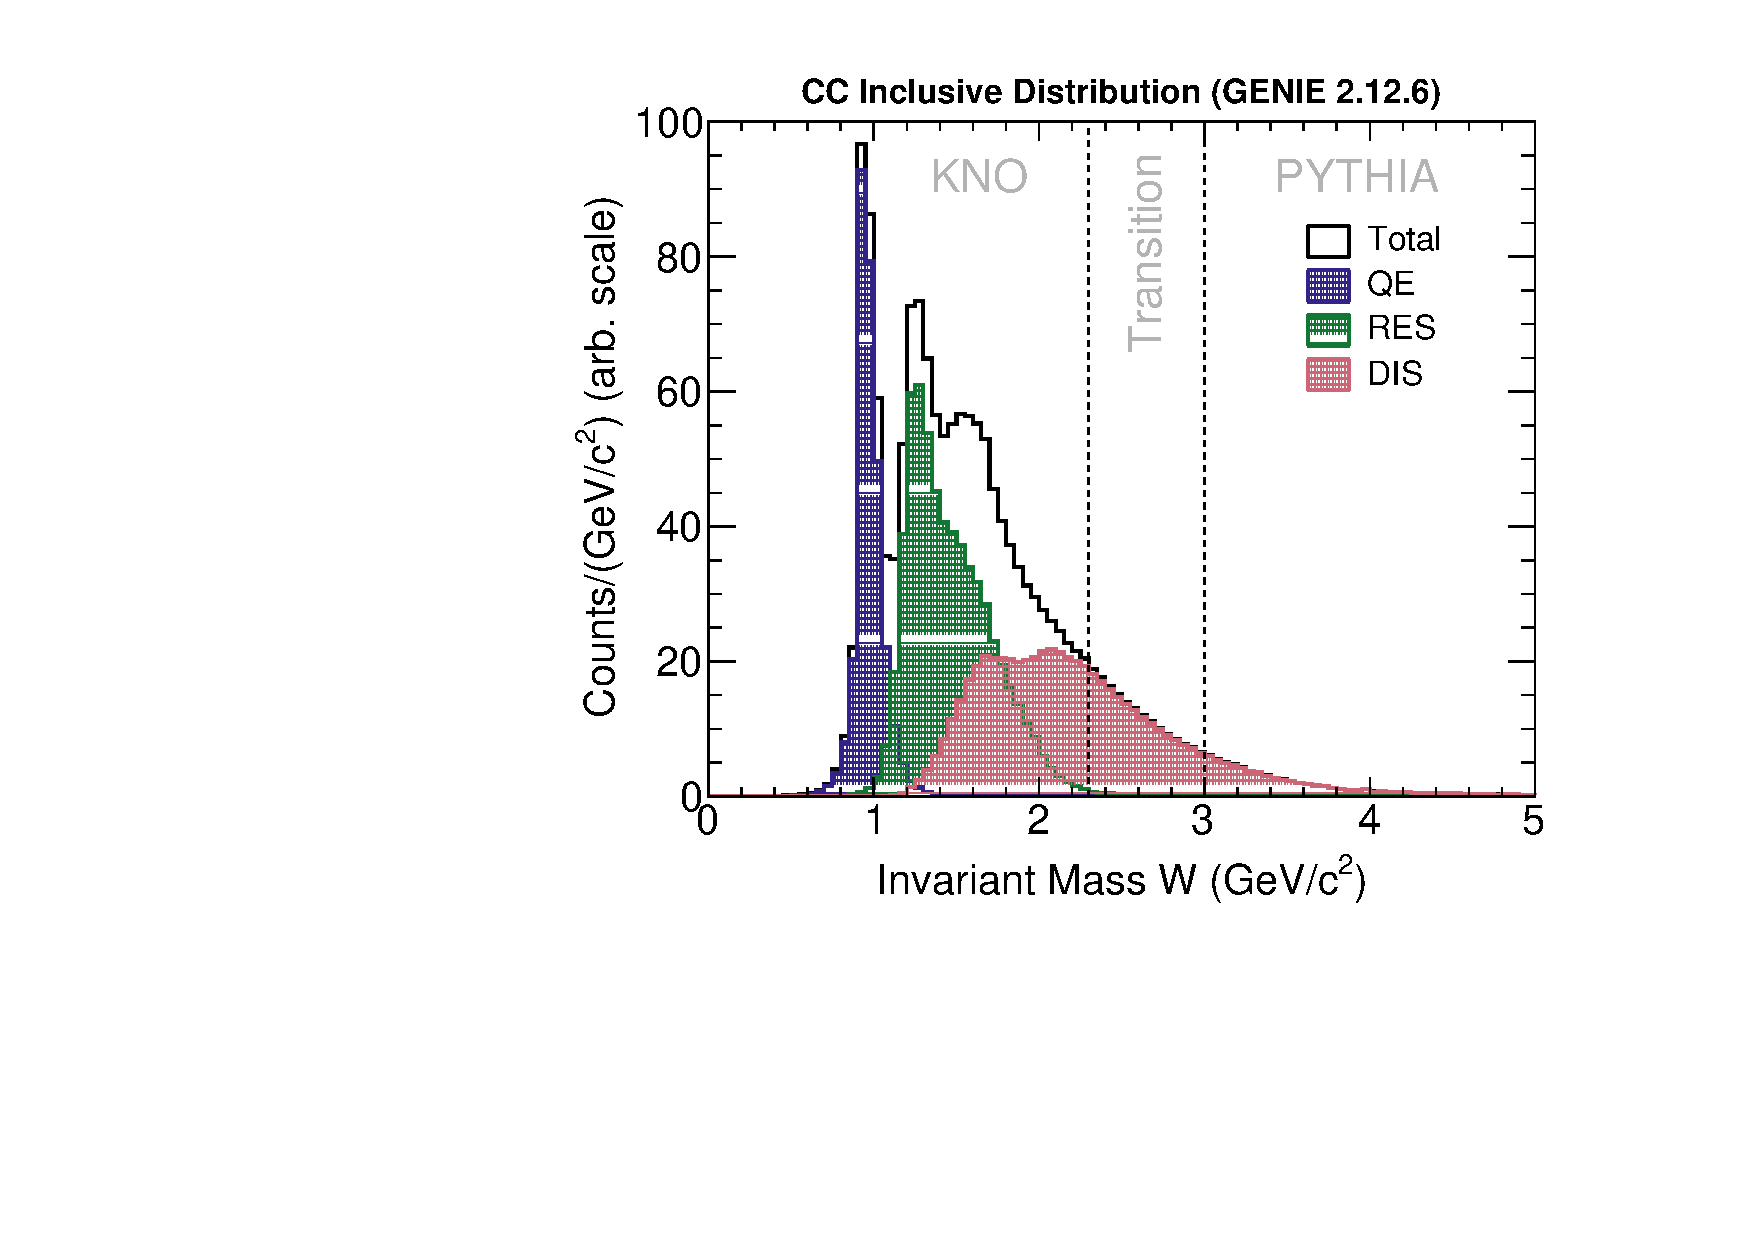
\includegraphics[width=0.8\textwidth]{05dataAsimulation/figures/WdistribGENIE.pdf}}%
  \caption{Invariant mass distribution $W$ of the charged-current antineutrino inclusive interactions on scintillator in GENIE 2.12.6, using the MINERvA antineutrino flux. The left blue region shows quasi-elastic scattering (QE), the middle green region represents resonance interactions (RES), and the right red region is deep inelastic scattering (DIS). The overlap between RES and DIS represents the transition region. The dashed lines split the $W$~distribution into the KNO-only region on the left, the PYTHIA-only region on the right, and the transition region in the middle. }
  %[short caption] {long caption}
  \label{fig:WdistribGENIE}
\end{figure}

% W distribution of ν µ-water target interaction in GENIE. For the flux, we use an atmospheric ν µ neutrino spectrum. Left red hatched region is quasi-elastic scattering, middle hatched region is resonance interactions, and right green hatched region is from DIS. The W distribution can be splitted to three regions, KNO scaling-baased model only region, PYTHIA only region, and the transtion region.

In contrast to the community definition of the DIS kinematic region of \mbox{$W >$ 2 GeV/$c^2$} and \mbox{$Q^2 >$ 1 (GeV/$c$)$^2$}, GENIE treats any non-resonant inelastic events as DIS. The antineutrino initially interacts with a single quark which then proceeds to hadronise, resulting in multiple hadrons in the final state. 

GENIE's DIS cross-section is calculated at the fully partonic level, accounting for the Bodek-Yang non-perturbative corrections to parton distribution functions (PDFs) as $Q^2$ decreases \cite{BodekYang_2003, BODEK2005113}, such as in the non-resonant pion production transition region described above. The Bodek-Yang model \cite{BodekYang_2003, BODEK2005113} also modifies the nuclear structure functions to incorporate nuclear effects as a function of Bjorken $x$, reflecting differences between nuclear and free nucleon structure functions, such as shadowing. Specifically, it utilises the parameterisations of charged lepton DIS measurements of $F_2^{\text{d}}/F_2^{\text{free}}$ and $F_2^{\text{Fe}}/F_2^{\text{d}}$, treating the axial and vector modifications equivalently. The same correction is applied to all nuclei.
%Bodek-Yang: https://arxiv.org/abs/hep-ex/0210024

%https://www.sciencedirect.com/science/article/pii/S0920563202017553
%Target mass correction is a kinematic correction where the mass of the target modifies the scattering kinematics and therefore the DIS structure functions. The higher twist correction is a dynamic correction due to non-perturbative parton-parton correlations. 

%https://arxiv.org/abs/0904.4043
The Andreopoulous-Gallagher-Kehayias-Yang (AGKY) model describes the hadronisation process in GENIE \cite{AGKY_Yang_2009}. In the AGKY model, the Koba-Nielsen-Olesen (KNO) model~\cite{KNO_KOBA1972317} is used for the \mbox{$W_{\text{min}} \leq $ 2.3 GeV/$c^2$} invariant mass, whereas the PYTHIA/JET\-SET~\cite{Pythia_Sjostrand_2001} program is utilised in the \mbox{$W_{\text{max}} > $ 3.0 GeV/$c^2$} region. The transition region $W_{\text{min}} < W \leq W_{\text{max}}$ is smooth as the fraction of PYTHIA hadronised events increases from 0\% to 100\% (and vice versa for KNO).

% AGKY: https://arxiv.org/abs/0904.4043
% KNO: https://www.sciencedirect.com/science/article/abs/pii/0550321372905512
% PYTHIA/JETSET: https://arxiv.org/abs/hep-ph/0010017

The KNO phenomenological model \cite{KNO_KOBA1972317} uses an empirical expression tuned to the Fermilab 15-foot bubble chamber neutrino-nucleon data to determine the hadron multiplicity \cite{AGKY_Yang_2009}. It selects particle content up to the multiplicity, generally a nucleon and any number of kinematically available low-mass mesons, e.g. $\pi$ and $K$. Finally, it partitions the available invariant mass $W$ among the generated hadrons to assign momenta. 

PYTHIA/JETSET \cite{Pythia_Sjostrand_2001} is a standard tool for the generation of high-energy collisions tuned to the BEBC data, spanning models for few-body hard processes to complex multihadronic final states. In the AGKY model, the PYTHIA region is not accessed until neutrino energy of approximately 3~GeV, and its contribution is equal to the one of KNO at around 9~GeV \cite{AGKY_Yang_2009}.
% Lund fragmentation function
% contains a library of hard pro- cesses and models for initial- and final-state parton showers, multiple parton-parton interactions, beam remnants, string fragmentation and particle decays.
% Tuned by NUX (MC generator for NOMAD)

%make figure like this 
%https://www.google.com/url?sa=i&url=https%3A%2F%2Fwww.researchgate.net%2Ffigure%2Fcolor-online-W-distribution-of-n-m-water-target-interaction-in-GENIE-For-the-flux-we_fig1_269635957&psig=AOvVaw3zlHm07k8xdJM4BFVcNKjs&ust=1700841191881000&source=images&cd=vfe&opi=89978449&ved=0CBIQjRxqFwoTCICvnqq92oIDFQAAAAAdAAAAABAE


\subsection{Final-state interactions}

Final-state interactions (FSI) occur as particles produced via the initial interaction traverse the nucleus to exit it. These interactions can change the final-state particle kinematics as well as the number of particles seen in the final state. GENIE models the FSI of nucleons and pions using intranuclear cascade simulation called INTRANUKE \cite{OGIntranuke_PhysRevD.45.743, RevisionIntranuke}. This analysis uses the effective data-driven model $hA$ \cite{genie_ANDREOPOULOS201087, genie_andreopoulos2015}. 

% OG intranuke: https://journals.aps.org/prd/abstract/10.1103/PhysRevD.45.743
% Revised intranuke: https://www.actaphys.uj.edu.pl/fulltext?series=Reg&vol=40&page=2445

The $hA$ implementation simulates the full cascade from a single effective interaction. It relies on the mean free path of the hadron to determine the probability that the FSI occurs. The interaction type, such as absorption, charge-exchange, elastic or inelastic scattering, relies on the external data, specifically cross-sections of ${\pi}^{+}$ and $p$ on \mbox{${}^{56}$Fe~\cite{genie_ANDREOPOULOS201087,genie_andreopoulos2015}}. Cross-sections are scaled by $A^{2/3}$ to predict FSI for other nuclei, and the isospin symmetry can be utilised to allow for predictions for $n$, $\pi^0$, and $\pi^-$. Furthermore, GENIE applies the FSI to the hadronic products of the interactions only, therefore the final-state muons are not affected.


%S. Dytman. INTRANUKE-hA. In AIP Conf Proc, volume 896, pages 178{184, 2007.
%https://arxiv.org/pdf/1510.05494.pdf

\begin{figure}[b!]
  \centering
  {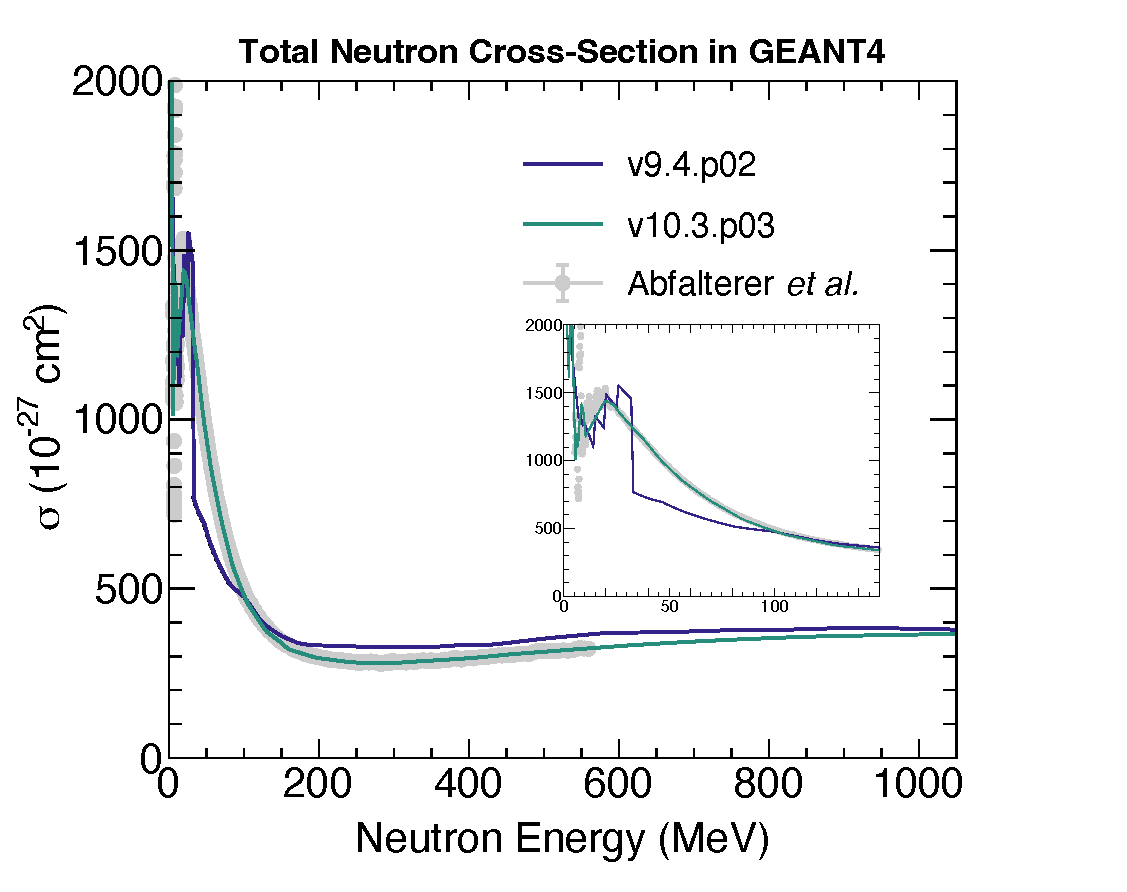
\includegraphics[width=0.8\textwidth]{05dataAsimulation/figures/totalNeutronXsec_wcloseup.pdf}}%
  \caption{Total neutron cross-section simulated by two different versions of GEANT4, v9.4.p02 and v10.3.p03, with overlayed Abfalterer \textit{et al.}~data~\cite{Abfalterer_PhysRevC.63.044608}. The older version of GEANT4 v9.4.p02 simulation shows significant disagreement with the Abfalterer \textit{et al.} data, whereas the newer version v10.3.p03 agrees with the data well. The insert shows the low neutron energy (0--200 MeV) behaviour of the two simulations versus data. }
  %[short caption] {long caption}
  \label{fig:neutronXsec}
\end{figure}

\section{Detector simulation}
Detector simulation models the propagation and the energy loss of the final-state particles through the MINERvA detector. Furthermore, it also accounts for the incidental activity in the detector via data overlay and employs the readout simulation to convert the energy deposits to simulated hits which can then be reconstructed.

\subsection{Particle propagation}
\label{sec:particleProp}

Particle propagation through the MINERvA detector uses the GEANT4 (GEometry ANd Tracking) software version 9.4.p02~\cite{Geant4_AGOSTINELLI2003250, Geant4_1610988}. The GEANT4 simulation proceeds in steps to determine if and how the final-state particles interact with a detailed description of MINERvA's geometry. The steps within a material are proposed by randomly sampling from the interaction length distributions implied by the interaction cross-sections for each process that applies to the particle. Based on the shortest step length, the particle either interacts or moves into a new material. Similarly, if an interaction produces secondary particles, their propagation is also simulated by GEANT4.

% Geant4: https://www.sciencedirect.com/science/article/pii/S0168900203013688
% Geant4: https://ieeexplore.ieee.org/document/1610988

The majority of interactions producing visible particles in the MINERvA detector come from the inelastic interactions. The inelastic hadron interactions in the detector use the QGSP\_BERT physics list, which employs the Bertini cascade (BERT) \cite{Bertini1963_PhysRev.131.1801,Guthrie:1968ue, Bertini1969_PhysRev.188.1711,BERTINI1971670} for particles with momentum less than \mbox{10 GeV/$c$} \cite{BertiniGeant4_heikkinen2003bertini}. For hadrons with momentum larger than \mbox{10 GeV/$c$}, GEANT4 uses the quark-gluon string precompound (QGSP) \cite{QGSP_folger2003string}. Other processes such as electromagnetic interactions or particle decays use the default modules of GEANT4. The particle propagation simulation ends with energy deposits and their associated timings along the track and at the end of the interaction step.

% Bertini cascade 1963: https://journals.aps.org/pr/abstract/10.1103/PhysRev.131.1801
% Bertini cascade 1968: https://www.sciencedirect.com/science/article/pii/0029554X68900542?via%3Dihub
% Bertini cascade 1969: https://journals.aps.org/pr/abstract/10.1103/PhysRev.188.1711
% Bertini cascade 1971: https://www.sciencedirect.com/science/article/pii/037594747190710X?via%3Dihub
% GEANT4 Bertini cascade: https://arxiv.org/abs/nucl-th/0306008v1
% QGSP in  GEANT4: https://arxiv.org/abs/nucl-th/0306007 

% Neutron is CV
% proton and pion just systematics
% neutron vs proton vs pion vs elastic
% reweight for neutron inelastic cross section
Furthermore, MINERvA reweights the events to modify the total neutron cross-section to match the Abfalterer \textit{et al.} \cite{Abfalterer_PhysRevC.63.044608} high-precision neutron scattering data which the newer versions of GEANT4 such as 10.3.p03 agree with \cite{Elkins2019_PhysRevD.100.052002}. The two GEANT4 total neutron cross-section simulations are compared to the Abfalterer \textit{et al.} data in Figure \ref{fig:neutronXsec}. The neutron interaction cross-section is increased via weighting up events with shorter tracks and weighting down events with longer tracks (and vice versa) while keeping the total number of (anti)neutrino events constant. A similar technique is used to evaluate the systematic uncertainties of the proton, pion and neutron interaction cross-sections and is further discussed in Chapter~\ref{ch:systematics}.


% MINERvA neutron reweight: https://journals.aps.org/prd/pdf/10.1103/PhysRevD.100.052002
% Abfalterer data: https://journals.aps.org/prc/abstract/10.1103/PhysRevC.63.044608

% MINERvA comparison Abfalterer vs Geant4: https://minerva-docdb.fnal.gov/cgi-bin/sso/RetrieveFile?docid=16284&filename=Kleykamp_2017-10-11_XsecNeutronOnX.pdf&version=3

% Systematics!! For example, for total inelastic cross-section for protons and pions, the variation is 10\% in carbon and hydrocarbon, 15\% in iron and 20\% in lead. Similarly, the neutron interaction cross-section is reweighted 
%https://minerva-docdb.fnal.gov/cgi-bin/sso/RetrieveFile?docid=7532&filename=dytman-hadr-uncert-27apr12.pdf&version=2


\subsection{Data overlay}
Additional effects such as particles produced in the rock between the NuMI beam and the detector, and overlapping (anti)neutrino interactions are not directly simulated. Instead, the MC hits are overlaid with data corresponding to random beam spills appropriate to the time periods in the simulation \cite{dataOverlay,TiceThesis2014}. The inserted data is flagged, ensuring it is not considered a signal candidate in the analysis.

% Internal MINERvA doc: https://minerva-docdb.fnal.gov/cgi-bin/sso/ShowDocument?docid=6032
% Tice thesis for data overlay/detector simulation: https://rucore.libraries.rutgers.edu/rutgers-lib/42462/

\subsection{Readout simulation}

Both the true deposits and timing need to be decalibrated to reconstruct the MC using the same methods as the data. First, all dead channels coming from the data overlay detector readout window are masked from the readout to account for the detector dead time and dead channels \cite{MarshallThesis2016}. 

% Marshall thesis dead channels: https://inspirehep.net/files/fd4468d48e6f7305f39526329836cf52
% Marshall internal detector simulation 101: https://minerva-docdb.fnal.gov/cgi-bin/sso/ShowDocument?docid=11234}

The energy deposited in the scintillator is converted into light yield using Birks' law \cite{Birks:1951boa}. The number of photoelectrons incident on the photomultiplier tube (PMT), which takes into account the attenuation of light in the fibres and additional smearing, is amplified using the gain of the PMT. The simulation also includes electronic noise and cross-talk. Finally, the photoelectrons are translated into raw ADC counts using the known analog-to-digital response \cite{WolcottThesis2015}.

% Wolcott thesis energy deposits to ADCs: https://www.osti.gov/biblio/1226351/

The simulated hit time is decalibrated by rounding to the nearest resolution width of the front-end-board (FEB) clock time. The known FEB offset and the travel time of photons to the PMT given the location of the hit along the scintillator strip is also added to the hit time and further smeared \cite{MarshallThesis2016}. 

% Marshall thesis time decalibration: https://inspirehep.net/files/fd4468d48e6f7305f39526329836cf52

% Birks law: https://iopscience.iop.org/article/10.1088/0370-1298/64/10/303
% Cross-talk



%the propagation and interaction or decay of the final state particles through the MINERvA detector.
 %This also includes simulating any secondary particles produces %from these interactions.

%This includes simulation o


%particle propagation
%data overlay
%readout simnulation
%mic track mathich efficiency weight
%particle  propagation weight





%- GENIE neutrino interaction simulation 
%- MINERvA interaction model reweighting
%- Detector simulation
%- simulation - reconstructed MC, truth
%- model 
